\section{Representación geométrica}

Para ver cómo funciona  el SVD a nivel geométrico, vamos a enunciar algunos lemas y observaciones. A continuación, los ilustraremos con un ejemplo numérico y su representación gráfica.\\

\begin{lemma}Las transformaciones ortogonales son isometrías, en el sentido de que preservan la norma de los vectores.
\end{lemma}

\begin{proof} Por definición, las aplicaciones ortogonales preservan el producto escalar. Como tanto la longitud (norma) de un vector como el ángulo entre dos vectores se definen a partir del producto escalar, por definición, la aplicación tiene que ser isométrica, es decir, conservará la distancia entre dos puntos.
\end{proof}

\begin{lemma} Una matriz cuyas únicas entradas no nulas son valores no negativos en la diagonal es, geométricamente, un escalado axial.
\end{lemma}

\begin{proof} Vamos a usar la matriz $\begin{pmatrix}
			\sigma_1 &        & 0        \\
			         & \ddots &          \\
			0        &        & \sigma_n
		\end{pmatrix}$ y un vector $\begin{pmatrix}
			x_1    \\
			\vdots \\
			x_n
		\end{pmatrix},$ siendo que $\sigma_1 \geq \dots \geq \sigma_n$.
	\[\begin{pmatrix}
			\sigma_1 &        & 0        \\
			         & \ddots &          \\
			0        &        & \sigma_n
		\end{pmatrix}
		\begin{pmatrix}
			x_1    \\
			\vdots \\
			x_n
		\end{pmatrix}
		=
		\begin{pmatrix}
			\sigma_1 x_1 \\
			\vdots       \\
			\sigma_n x_n
		\end{pmatrix}
	\]

	Se observa que el crecimiento de cada elemento ocurre de acuerdo a su elemento correspondiente en la diagonal, y por lo tanto, dado un vector cualquiera, los elementos de la diagonal producen escalados axiales. Si la matriz no fuese cuadrada, el resultado tendría simplemente algunos ceros adicionales (o algunas dimensiones no se reflejarían en la imagen).
\end{proof}

\begin{theorem} La imagen de la esfera unidad bajo una aplicación $A$ será un elipsoide cuyos semiejes tienen longitudes iguales a los valores singulares de $A$, y direcciones que cambian respecto a los ejes de coordenadas originales de una manera que puede medirse mediante el cambio de base generado por las matrices $U$ y $V^t$, las cuales se obtienen al realizar SVD.
\end{theorem}

\begin{proof} Para empezar, gracias al SVD, podemos descomponer la matriz de la aplicación en cuestión en el producto de dos matrices ortogonales y una matriz diagonal. Como hemos demostrado que el efecto de una aplicación con una matriz  diagonal no negativa es una deformación axial, la matriz $\Sigma$ del SVD causará un escalado axial a la esfera. Por lo tanto la imagen de $\Sigma$ será un elipsoide, ya que el escalado axial de una esfera es un elipsoide. Como tanto $V^t$ como $U$ son ortogonales, no pueden causar un escalado, ya que como hemos demostrado, son isometrías, y por lo tanto, sus imágenes conservarán el mismo tipo de forma que eran antes de aplicárselas, es decir, una esfera y un elipsoide respectivamente. Por lo tanto, la imagen de una esfera será, en efecto, un elipsoide.\\
	De una manera más formal, si tenemos un objeto geométrico $S=\left\lbrace x\in \mathbb{R}^n:||x||=1 \right\rbrace$, que es la esfera unidad, se puede encontrar su imagen por $A$ como:
	\begin{enumerate}
		\item $V^tS=S$, ya que $V^t$ es una isometría, y por lo tanto, mantiene las distancias.
		\item $\Sigma S=\left\lbrace(\sigma_1x_1,\sigma_2x_2,\dots,\sigma_nx_n):\sum_{i=1}^{n}(x_i)^2=1\right\rbrace$. Si sustituimos $y_i=\sigma_ix_i$, entonces obtenemos que $S'=\left\lbrace y\in\mathbb{R}:\sum_{i=1}^{n}(\frac{y_i}{\sigma_i})^2=1\right\rbrace$, la cual es la ecuación estándar del elipsoide de semiejes $\sigma_i e_i$, siendo $S'$ la imagen de S por la aplicación $\Sigma$.
		\item $US'$ correspondería entonces a un elipsoide de semiejes $\sigma_iUe_i$. Los vectores $\{ Ue_i\}$ forman una base ortonormal porque $U$ es una isometría.
	\end{enumerate}
	Por lo tanto, se puede ver que la imagen por $A$ de una esfera unidad $S$ será un elipsoide.
\end{proof}

Por último, para ilustrar la representación geométrica del SVD, vamos a desarrollar un ejemplo utilizando la matriz
\[
	A =
	\begin{pmatrix}
		\frac{\sqrt2}{2} & \frac{-\sqrt2}{2} \\
		\frac{\sqrt2}{2} & \frac{\sqrt2}{2}  \\
		\frac{\sqrt6}{2} & \frac{-\sqrt6}{2}
	\end{pmatrix}
\]

Lo primero que vamos a hacer es encontrar el resultado de $A^tA$, por lo que vamos a realizar la operación:
\[
	B=
	\begin{pmatrix}
		\frac{\sqrt2}{2}  & \frac{\sqrt2}{2} & \frac{\sqrt6}{2}  \\
		\frac{-\sqrt2}{2} & \frac{\sqrt2}{2} & \frac{-\sqrt6}{2} \\
	\end{pmatrix}
	\begin{pmatrix}
		\frac{\sqrt2}{2} & \frac{-\sqrt2}{2} \\
		\frac{\sqrt2}{2} & \frac{\sqrt2}{2}  \\
		\frac{\sqrt6}{2} & \frac{-\sqrt6}{2}
	\end{pmatrix}
	=
	\begin{pmatrix}
		\frac{5}{2}  & \frac{-3}{2} \\
		\frac{-3}{2} & \frac{5}{2}
	\end{pmatrix}
\]
La razón por la que hacemos $A^tA$ en lugar de $AA^t$ es porque la matriz $AA^t$ es una matriz $3\times3$ con un autovalor nulo. El resultado final sería el mismo, pero la complejidad del cálculo más costoso (la diagonalización de la matriz) sería mayor.

Una vez hemos calculado la matriz $B$, la vamos a utilizar para obtener sus autovectores, que son necesarios para calcular la matriz $V^t$. Primero calcularemos los autovalores, que se obtienen del polinomio característico, el cual obtendremos a partir de la siguiente matriz $C$:
\[
	C=B-\lambda I=
	\begin{pmatrix}
		\frac{5}{2}-\lambda & \frac{-3}{2}        \\
		\frac{-3}{2}        & \frac{5}{2}-\lambda
	\end{pmatrix}
\]
\[
	det(C)=\frac{25}{4}-5\lambda+\lambda^2-\frac{9}{4}=\lambda^2-5\lambda+4
\]
\[
	\lambda=\frac{5\pm\sqrt{5^2-16}}{2}=\frac{5\pm\sqrt9}{2}=\frac{5\pm3}{2}
\]
\[
	\lambda = \frac{5+3}{2}=4;\lambda=\frac{5-3}{2}=1
\]
Una vez tenemos los autovalores ($4$ y $1$), vamos a hallar los autovectores calculando el núcleo de $B-\lambda I$, es decir, restando a la matriz $B$ la identidad por cada autovalor:
\[
	B-4I=
	\begin{pmatrix}
		\frac{5}{2}  & \frac{-3}{2} \\
		\frac{-3}{2} & \frac{5}{2}
	\end{pmatrix}
	-
	\begin{pmatrix}
		4 & 0 \\
		0 & 4
	\end{pmatrix}
	=
	\begin{pmatrix}
		\frac{-3}{2} & \frac{-3}{2} \\
		\frac{-3}{2} & \frac{-3}{2}
	\end{pmatrix}
\]
Por lo tanto, la ecuación del autoespacio correspondiente al autovalor $4$ será $x+y=0$ y un autovector suyo será $\begin{pmatrix}
		1 \\
		-1
	\end{pmatrix}$
que, normalizado, es $\begin{pmatrix}
		\frac{\sqrt2}{2} \\
		\frac{-\sqrt2}{2}
	\end{pmatrix}$.
Calculamos a continuación el segundo autovector:
\[
	B-I=
	\begin{pmatrix}
		\frac{5}{2}  & \frac{-3}{2} \\
		\frac{-3}{2} & \frac{5}{2}
	\end{pmatrix}
	-
	\begin{pmatrix}
		1 & 0 \\
		0 & 1
	\end{pmatrix}
	=
	\begin{pmatrix}
		\frac{3}{2}  & \frac{-3}{2} \\
		\frac{-3}{2} & \frac{3}{2}
	\end{pmatrix}
\]
De aquí sabemos ahora que la ecuación del autoespacio correspondiente al autovalor $1$ será $x-y=0$, por lo tanto el autovector será $\begin{pmatrix}
		1 \\
		1
	\end{pmatrix}$
que una vez normalizado se escribe $\begin{pmatrix}
		\frac{\sqrt2}{2} \\
		\frac{\sqrt2}{2}
	\end{pmatrix},$
y por lo tanto ya conocemos $V^t$, que será igual a $\begin{pmatrix}
		\frac{\sqrt2}{2} & \frac{-\sqrt2}{2} \\
		\frac{\sqrt2}{2} & \frac{\sqrt2}{2}
	\end{pmatrix}$

A partir de esta, vamos a calcular la matriz $U$, utilizando los autovectores normalizados y la matriz $\Sigma$, en cuya diagonal están las raíces de los autovalores:
\[
	u_1=\frac{1}{2}Av_1=\frac{1}{2}\begin{pmatrix}
		\frac{\sqrt2}{2} & \frac{-\sqrt2}{2} \\
		\frac{\sqrt2}{2} & \frac{\sqrt2}{2}  \\
		\frac{\sqrt6}{2} & \frac{-\sqrt6}{2}
	\end{pmatrix}
	\begin{pmatrix}
		\frac{\sqrt2}{2} \\
		\frac{-\sqrt2}{2}
	\end{pmatrix}
	=\frac{1}{2}
	\begin{pmatrix}
		1 \\
		0 \\
		\sqrt3
	\end{pmatrix}
	=
	\begin{pmatrix}
		\frac{1}{2} \\
		0           \\
		\frac{\sqrt3}{2}
	\end{pmatrix}
\]
\[
	u_2=\frac{1}{1}Av_2=\begin{pmatrix}
		\frac{\sqrt2}{2} & \frac{-\sqrt2}{2} \\
		\frac{\sqrt2}{2} & \frac{\sqrt2}{2}  \\
		\frac{\sqrt6}{2} & \frac{-\sqrt6}{2}
	\end{pmatrix}
	\begin{pmatrix}
		\frac{\sqrt2}{2} \\
		\frac{\sqrt2}{2}
	\end{pmatrix}
	=
	\begin{pmatrix}
		0 \\
		1 \\
		0
	\end{pmatrix}
\]
$u_3$ lo vamos a calcular utilizando el producto vectorial, ya que $u_1, u_2$ y $u_3$ tienen que formar una base ortonormal.

\[
	\begin{pmatrix}
		\frac{1}{2} \\
		0           \\
		\frac{\sqrt3}{2}
	\end{pmatrix}
	\times
	\begin{pmatrix}
		0 \\
		1 \\
		0
	\end{pmatrix}
	=
	\begin{vmatrix}
		i           & j & k                \\
		\frac{1}{2} & 0 & \frac{\sqrt3}{2} \\
		0           & 1 & 0
	\end{vmatrix}
	=
	\frac{k}{2}-\frac{\sqrt3}{2}i
\]
\[
	u_3=\begin{pmatrix}
		-\frac{\sqrt3}{2} \\
		0                 \\
		\frac{1}{2}
	\end{pmatrix}
\]
Por lo tanto la matriz $U=\begin{pmatrix}
		\frac{1}{2}      & 0 & -\frac{\sqrt3}{2} \\
		0                & 1 & 0                 \\
		\frac{\sqrt3}{2} & 0 & \frac{1}{2}
	\end{pmatrix}$. Como tenemos tanto $U$ como $V^t$ y las raíces de los autovalores, podemos decir que $\Sigma=\begin{pmatrix}
		2 & 0 \\
		0 & 1 \\
		0 & 0
	\end{pmatrix}$, comprobando que es correcto que $U\Sigma V^t=A$

Ahora vamos a analizar este ejemplo para ver cómo sería geométricamente lo que acabamos de resolver. Lo primero, vamos a ver qué hace cada matriz.

Las matrices tanto $V^t$ como $U$ representan un cambio de base ortonormal, ya que son ortogonales, y, por lo tanto, isometrías. Por su parte, la matriz $\Sigma$ representa un escalado axial. Lo que estamos haciendo cuando operamos un objeto geométrico $n$ en la base que es la matriz $V$ por la matriz $A$ es:\begin{enumerate}
	\item Paso el vector de la base canónica a la base descrita por la matriz $V$, que es la base en la que está $\Sigma$, al hacer $V^tn=n'$
	\item Calculo el escalado del vector al hacer $\Sigma n'=n''$, ambos descritos en las respectivas bases dadas por $V$ y $U$.
	\item Transformo el vector ya escalado de la base $U$ a la canónica al hacer $Un''$
\end{enumerate}
Es decir, la matriz $A$, geométricamente, escala y rota un vector (o un lugar geométrico). Esto podría ocurrir ya sea en la misma dimensión, pasando a una dimensión mayor, como es en el caso del ejemplo, o a una menor.

Para comprobar la corrección de nuestros cálculos (y realizar una representación gráfica), vamos a desarrollar el ejemplo anterior fijando una preimagen $n_1$ y calculando $An_1$ y $U\Sigma V^tn_1$.
\[
	n_1=\begin{pmatrix}
		2 \\
		0
	\end{pmatrix}; An_1=\begin{pmatrix}
		\frac{\sqrt2}{2} & \frac{-\sqrt2}{2} \\
		\frac{\sqrt2}{2} & \frac{\sqrt2}{2}  \\
		\frac{\sqrt6}{2} & \frac{-\sqrt6}{2}
	\end{pmatrix}
	\begin{pmatrix}
		2 \\
		0
	\end{pmatrix}
	=
	\begin{pmatrix}
		\sqrt2 \\
		\sqrt2 \\
		\sqrt6
	\end{pmatrix}
\]
\[
	U\Sigma V^tn_1=\begin{pmatrix}
		\frac{1}{2}      & 0 & -\frac{\sqrt3}{2} \\
		0                & 1 & 0                 \\
		\frac{\sqrt3}{2} & 0 & \frac{1}{2}
	\end{pmatrix}
	\begin{pmatrix}
		2 & 0 \\
		0 & 1 \\
		0 & 0
	\end{pmatrix}
	\begin{pmatrix}
		\frac{\sqrt2}{2} & \frac{-\sqrt2}{2} \\
		\frac{\sqrt2}{2} & \frac{\sqrt2}{2}
	\end{pmatrix}
	\begin{pmatrix}
		2 \\
		0
	\end{pmatrix}
	=
	\begin{pmatrix}
		\frac{1}{2}      & 0 & -\frac{\sqrt3}{2} \\
		0                & 1 & 0                 \\
		\frac{\sqrt3}{2} & 0 & \frac{1}{2}
	\end{pmatrix}
	\begin{pmatrix}
		2 & 0 \\
		0 & 1 \\
		0 & 0
	\end{pmatrix}
	\begin{pmatrix}
		\sqrt2 \\
		\sqrt2
	\end{pmatrix}
	=
\]
\[
	=
	\begin{pmatrix}
		\frac{1}{2}      & 0 & -\frac{\sqrt3}{2} \\
		0                & 1 & 0                 \\
		\frac{\sqrt3}{2} & 0 & \frac{1}{2}
	\end{pmatrix}
	\begin{pmatrix}
		2\sqrt2 \\
		\sqrt2  \\
		0
	\end{pmatrix}
	=
	\begin{pmatrix}
		\sqrt2 \\
		\sqrt2 \\
		\sqrt6
	\end{pmatrix}
\]
Podemos ver cómo obtenemos, en efecto, el mismo resultado al multiplicar $An_1$ y al calcular  $U\Sigma V^tn_1$, y que, como $U$ y $V^t$ son simplemente cambios de base, $\Sigma$ contiene toda la información sobre la deformación. En definitiva, SVD permite calcular y visualizar geométricamente la deformación de un objeto geométrico al aplicarle una aplicación lineal.

Por último, ilustramos este último ejemplo mostrando el proceso paso a paso.

\begin{figure}[h]
	\centering
	\begin{subfigure}{0.45\textwidth}
		\centering
		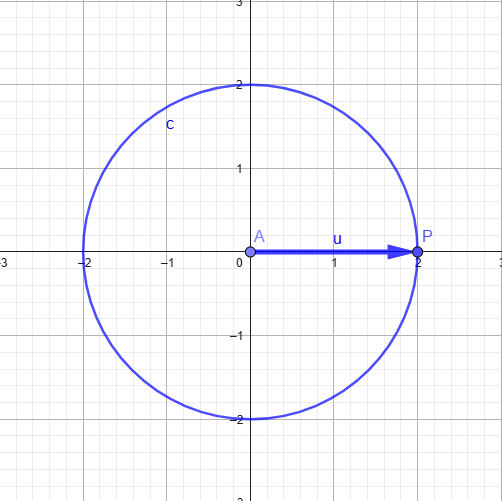
\includegraphics[width=\linewidth]{figures/Circulo 1.png}
		\caption{Vector original}
	\end{subfigure}
	\begin{subfigure}{0.45\textwidth}
		\centering
		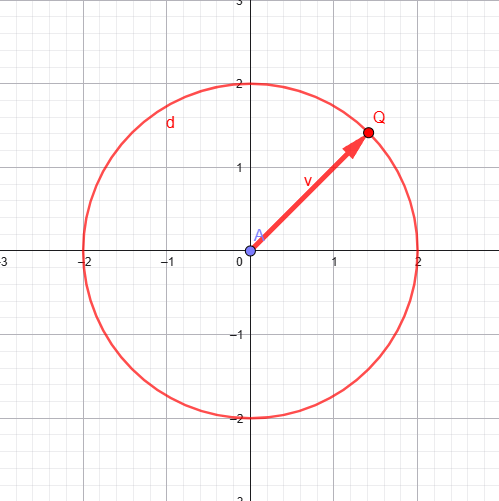
\includegraphics[width=\linewidth]{figures/Circulo 2.png}
		\caption{Vector en la nueva base}
	\end{subfigure}

	\begin{subfigure}{0.45\textwidth}
		\centering
		
\includegraphics[width=\linewidth]{Elipse.png}
		\caption{Vector deformado por la matriz obtenida por SVD}
	\end{subfigure}
	\begin{subfigure}{0.45\textwidth}
		\centering
		
\includegraphics[width=\linewidth]{Elipse 3d.png}
		\caption{Vector deformado pasado a la segunda base}
	\end{subfigure}
\end{figure}

